\chapter{Integer Grid Maps}
The necessary and sufficient conditions for a parametrization mapping to form a valid quad mesh on the mesh's 3D surface are:
\begin{enumerate}
\item Seamless Condition
\item Singular Points Condition
\item Consistent Orientation Condition
\end{enumerate}

\section{Seamless Condition}
The transition function $g_{ij}$ between two half-edges $e_i$ and $e_j$ on the parameterization domain that corresponds to the same surface edge that is part of a cut seam, has to be an integer-grid automorphism given by:
\begin{equation}\label{transition_g_ij}
\begin{split}
e_j = R^{r_{ij}}_{90^\circ}e_i + \vec{t}_{ij}
\end{split}
\end{equation}
Where  $r_{ij} \in \{0,1,2,3\}$ and $\vec{t}_{ij} \in \mathbb{Z}^2$. Figures \ref{fig:translation_req}, \ref{fig:angle_req} and \ref{fig:length_req} visually demonstrate the 3 requirements encoded by the seamless condition.
  
\begin{figure}[ht]
\centering
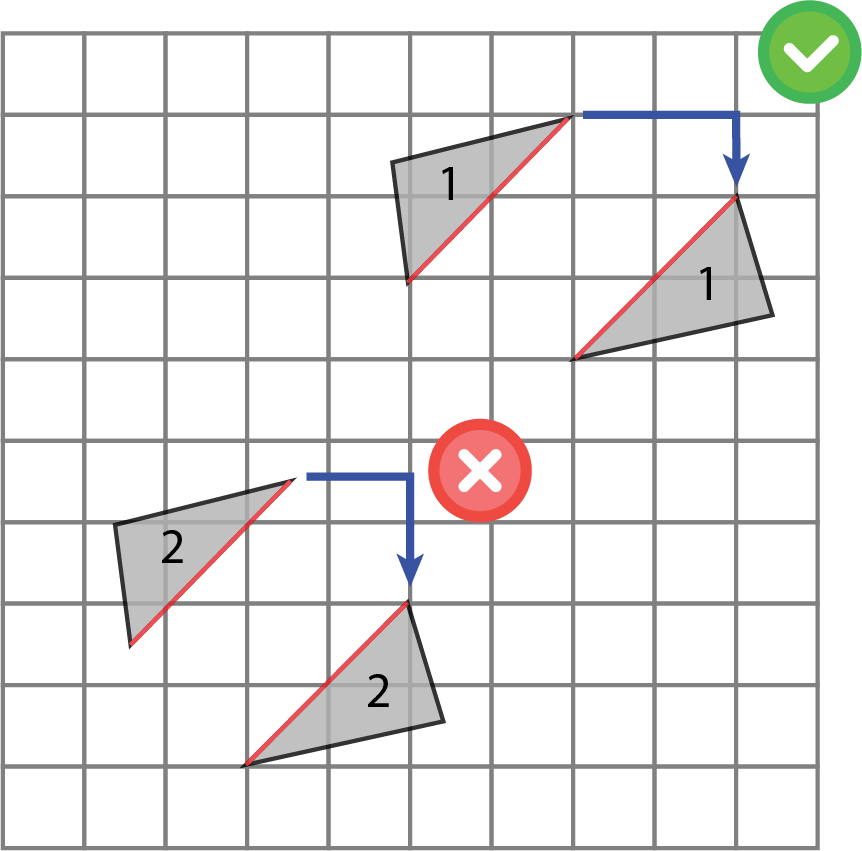
\includegraphics[width=9cm]{figures/seamless/translation.png}
\caption[The Translation Requirement]{The transition function $g_{ij}$, described by equation \ref{transition_g_ij}, should impose an integer translation between the two half edges.}
\label{fig:translation_req}
\end{figure}

\begin{figure}[ht]
\centering
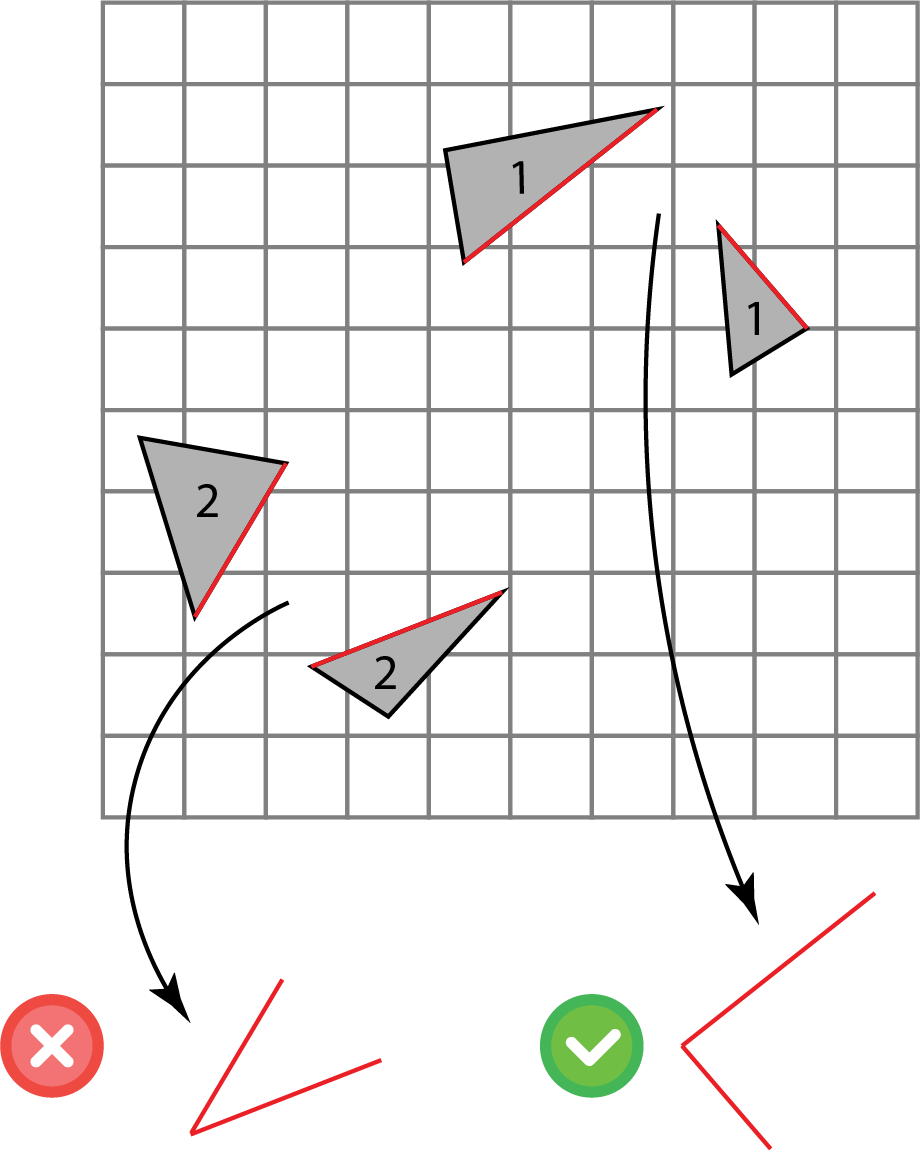
\includegraphics[width=9cm]{figures/seamless/angle.png}
\caption[The Angle Requirement]{The transition function $g_{ij}$, described by equation \ref{transition_g_ij}, should impose a $\frac{\pi}{2}k$ rotation between the two half edges.}
\label{fig:angle_req}
\end{figure}

\begin{figure}[ht]
\centering
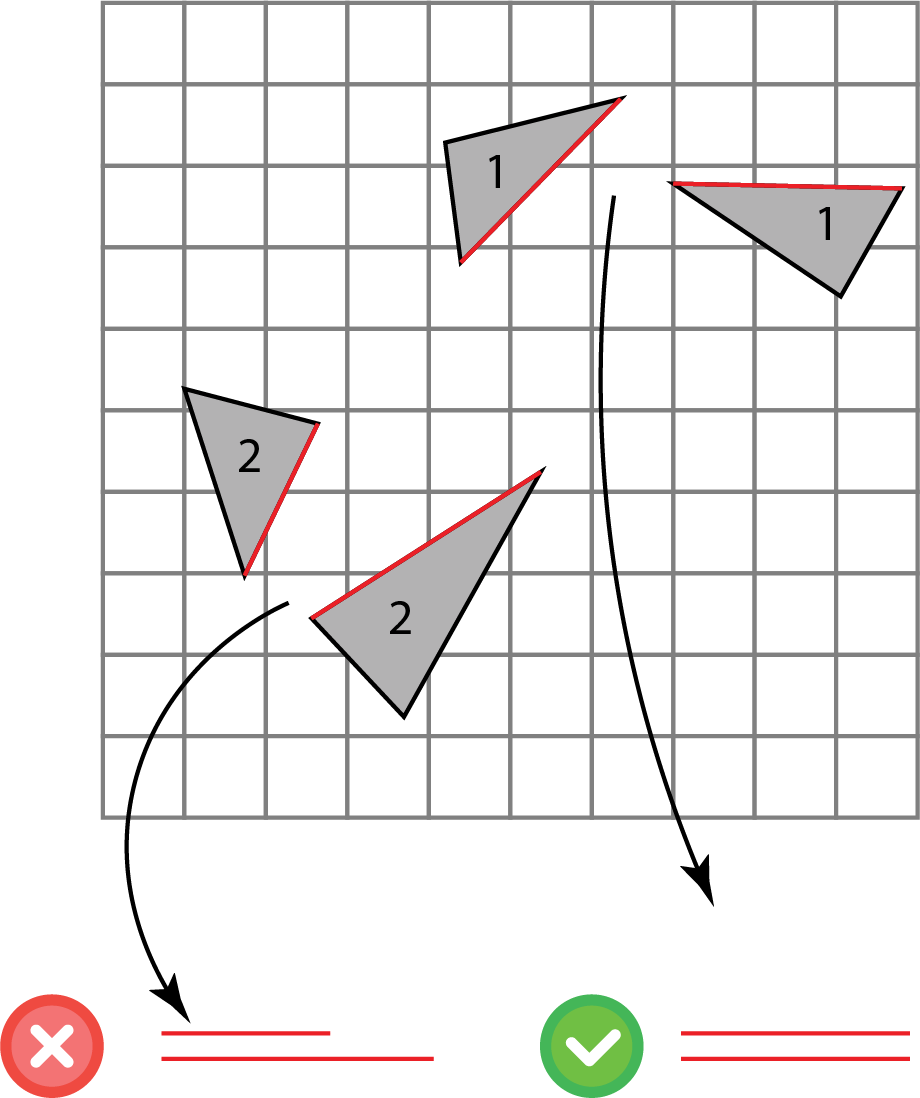
\includegraphics[width=9cm]{figures/seamless/length.png}
\caption[The Length Requirement]{The transition function $g_{ij}$, described by equation \ref{transition_g_ij}, should implicitly match the length of the two half edges.}
\label{fig:length_req}
\end{figure}

\section{Singular Points Condition}
All singular vertices, which are characterized by a non-zero angular defect on the parameterization domain, have to lie on integer locations. That is, given the set $S_i$ of all parameterization domain vertices that correspond to the same singular surface vertex $v_i$, we require that:
$$\forall u \in S_i: u \in \mathbb{Z}^2 $$
Figures \ref{fig:singular_points_req} demonstrate this condition visually.
  
\begin{figure}[ht]
\centering
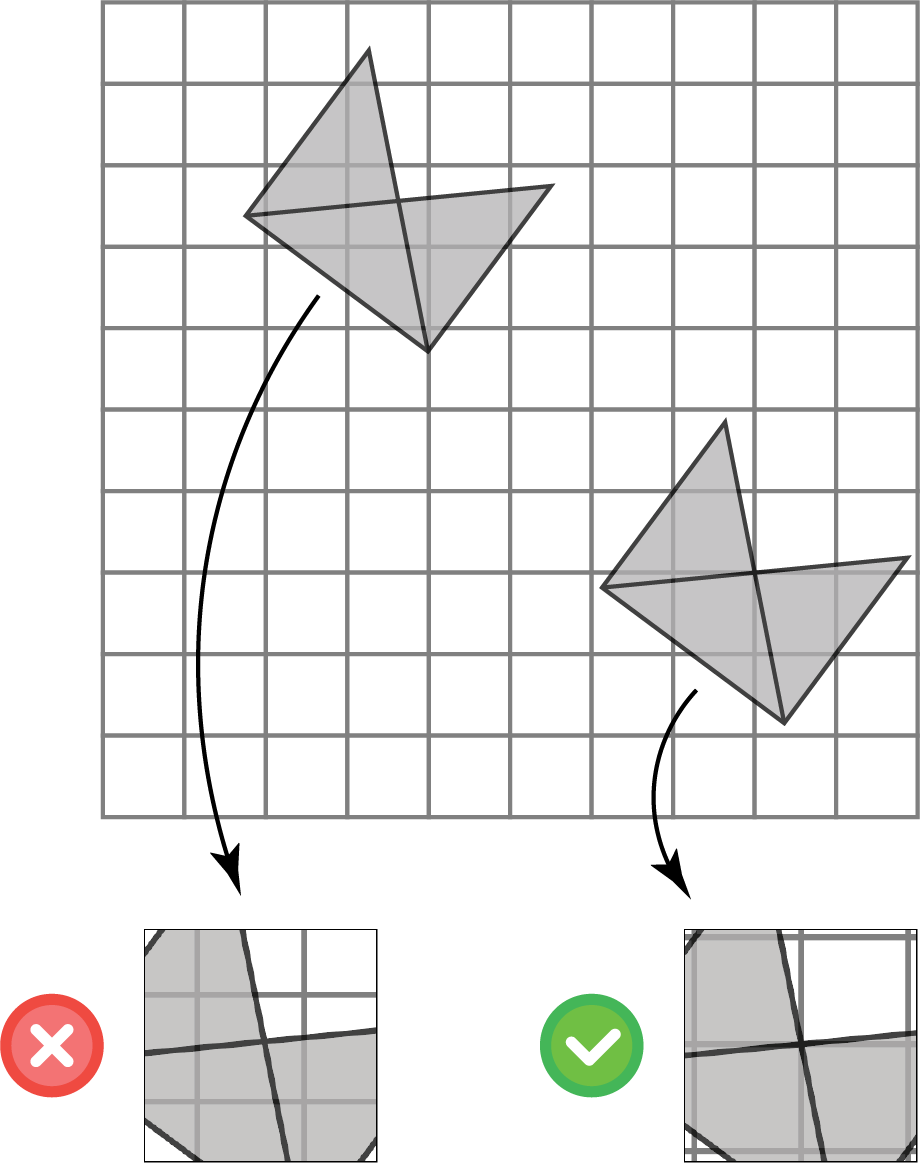
\includegraphics[width=9cm]{figures/singular_points/singularity.png}
\caption[The Singular Points Requirement]{All of the domain vertices that correspond to the same singular point should be positioned at a grid point (integer location).}
\label{fig:singular_points_req}
\end{figure}

\section{Consistent Orientation Condition}
All triangles on the parameterization domain should have the same orientation. That is, the transition function should not allow triangle.

\begin{figure}[ht]
\centering
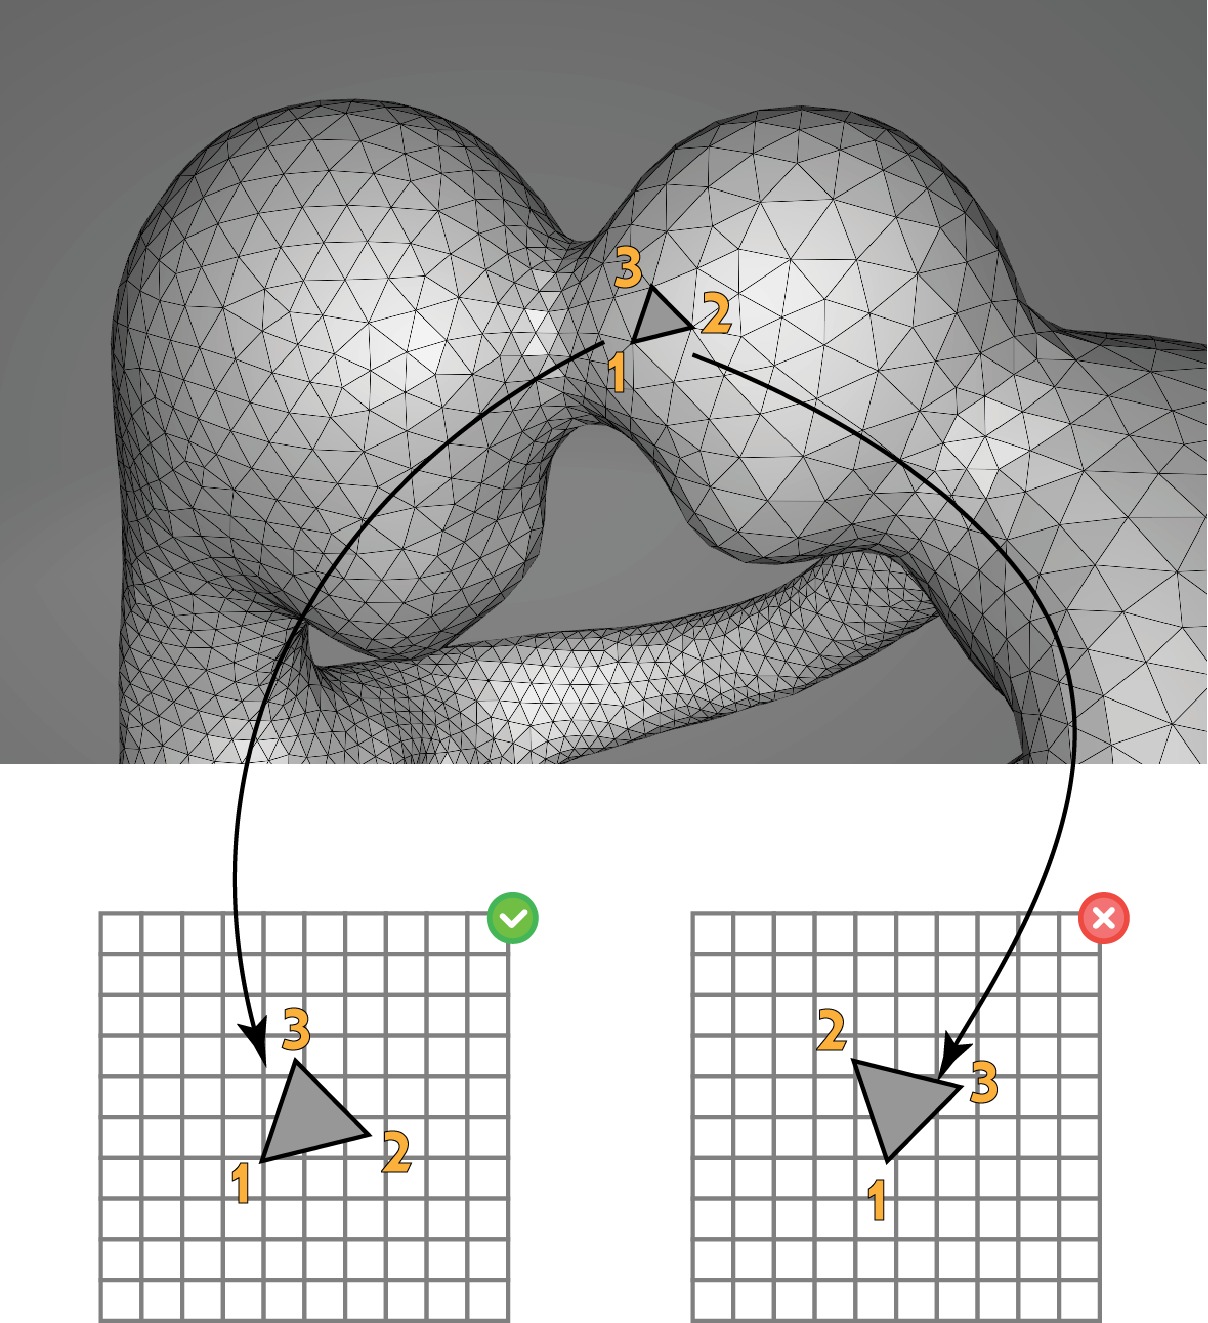
\includegraphics[width=9cm]{figures/orientation/orientation.png}
\caption[The Orientation Requirement]{The left triangle follows the same counter clockwise orientation as its image on the mesh's surface. On the other hand, the vertices of the triangle on the right follows a clockwise orientation.}
\label{fig:orientation_req}
\end{figure}